

%\documentclass{book}
\documentclass[12pt,a4paper]{report}

\usepackage[latin2]{inputenc}
\usepackage{amsfonts}
\usepackage[MeX]{polski}
\usepackage{verbatim}
\usepackage{graphicx}
\usepackage{fancyhdr}
\usepackage{booktabs}
\usepackage{xspace}
\usepackage{supertabular}
\usepackage{listings}
\usepackage{color}

\usepackage{caption}
\renewcommand{\captionfont}{\itshape}		% ewentualnie moze \bfseries

\definecolor{darkgray}{rgb}{0.95,0.95,0.95}
\lstset{language=Java}
\lstset{backgroundcolor=\color{white}}
\lstset{numbers=left, numberstyle=\tiny, stepnumber=1, numbersep=5pt}
\lstset{keywordstyle=\color{black}\bfseries\emph}
\lstset{basicstyle=\footnotesize}

\title{Badanie wydajno�ci system�w o architekturze SOA \\
 \large Praca magisterska
}
\author{Tomasz Duszka i Jakub Janczak}

\begin{document}

\pagenumbering{roman}

\thispagestyle{empty}
\begin{center}
Akademia G�rniczo - Hutnicza im. Stanis�awa Staszica w Krakowie \\
Wydzia� Elektrotechniki, Automatyki, Informatyki i Elektroniki \\
Katedra Informatyki
% \\ Akademii G�rniczo Hutniczej w Krakowie
\rule{\textwidth}{.1mm}
\end{center}

\begin{figure}[hkp!]
 \centering
% \includegraphics[width=50pt]{agh_znak}
 \includegraphics[bb=0 0 64 124]{agh_logo_kolor.png}
 \label{fig:orzel_agh}
\end{figure}

% \vskip 80pt
\begin{center}
{\bf \large Praca magisterska}
\vskip 10pt
{\bf \huge Badanie wydajno�ci system�w o architekturze SOA}
\end{center}

\vskip 60pt
\begin{center}
{\Large \bf Tomasz Duszka, Jakub Janczak}\\
\texttt{duszka@student.agh.edu.pl, janczak@student.agh.edu.pl}
\end{center}

\vskip 80pt
\begin{center}
{\bf
    Promotor: dr in�. Dominik Radziszowski
}
\end{center}

\vskip 60pt
\noindent
\rule{\textwidth}{.1mm}
\begin{center}
Krak�w, 2008
\end{center}


% \maketitle

\pagenumbering{arabic}

\newpage

%\linespread{1.3}		%1.3 dla interlinii 1.5

\tableofcontents

%\part{Wst�p}

We are limited\ldots

Despite the ,,Moore's law'' we are limited in computing s.
As the computers grow larger and larger, we have to be aware of the fact that the moment of ,,The highest limit'' is coming very quickly, and as a matter of fact we can't stave off it.
One of these problems is ,,memory problem''.
Giving memory devices greater size we have to combine it with increasing speed, what physics has proved is limited by the light speed.
Out-of-core researches are the answer for these problems. ,,Out-of-core'' - means that the problem can't be stored in normal \footnote{technologically-achievable} computer's memory and nowadays it's a possibility for scientists to achieve great computing goals on available computers.
But in many mathematics' opinion it could be the only way to use electrical computers in the future when we "touch the roof" in their abilities.

\emph{Out-of-core problems} are these which can't be whole stored in the memory in the one moment and could be quite big in our opinion.
For example there is a class of problems called Grand Challenge Applications which need about 100 gigabytes of data per run.\cite{grandc}
Thus it's obviously needed to fetch some data into the memory leaving the rest in the memory, process it as much as we can and then take another chunk from mass storage medias (~RAID matrices or similar~).

\subsection{Variety of OOC problems}
There are many kinds of OOC problems, some of them are:
\begin{itemize}
	\item{Big matrices operations ( inverting, multiplying, transpositioning etc. )}
	\item{Huge sets of equations solving ( also decompositions ) }
	\item{Processing great meshes ( rendering etc. )}
	\item{Data mining}
	\item{Out of core sorting}
	\item{Markov models out of core symbolic solving}

\end{itemize}
	
\subsection{Variation of abstract models}
There are three most common kinds of OOC's solve models used in parallel computing: \cite{kzajac1}
\begin{itemize}
%	\clearpage
	\item{General placement model} -- when the memory is available for all the processes and is stored in one BIG virtual file -- figure 1
	\begin{figure}[h!]
		\begin{center}
			\includegraphics{fig1.fig.eps}
			\caption{General placement model}
		\end{center}
	\end{figure}
	\item{Local placement model} -- every process has it's own portion of data ( own file ) in it's memory and the exchange of data is made by I/O operations ( which is unfortunately very low effective ) -- figure 2
	\begin{figure}[h!]
		\begin{center}
			\includegraphics{fig2.fig.eps}
			\caption{Local placement model}
		\end{center}
	\end{figure}
	\item{Partitioned-in-core model} --
	when we are lucky - problem can be logically divided, so the I/O operations aren't needed.
	The only problem is that the processes should have as much memory as one ,,problem chunk'' needs -- figure 3

	
	\begin{figure}[h!]
		\begin{center}
			\includegraphics{fig3.fig.eps}
			\caption{Partitioned-in-core placement model}
		\end{center}
	\end{figure}
	
\end{itemize}
\subsection{Parallel I/O problems}
As we could see the main problem with OOC problem ( esp. in 2nd case ) is I/O subsystem.
There are many ways to help computer in it's work.
They can be divided for groups ( using another levels of software and hardware ):
\begin{itemize}
	\item{Hardware ways} - consists of parallel device support, such as RAID. They are small scaled and they don't affect the software level
	\item{Parallel filesystems} - providing very efficient filesystem access as a part of High Throughput Computing. They should provide three services:
	\begin{itemize}
		\item{consistent namespace across the machine}
		\item{distribution of data across the disks or network stations}
		\item{some additional I/O links}
	\end{itemize}
	It's for example PVFS wich is striping all the data across multiple disks of different nodes in cluster.
	Doing it such a way we are able to create larger files with better bandwidth available, and without network speed problems ( "bottlenecks" ).
	It also supports 64-bit address space, so we are able to create really huge files.
	Another advantages of using PVFS are working in user-level space, good cooperation with MPI-IO and NASA support.\cite{pvfs}

	Another example of parallel filesystem is HDIOS which has been done by bypassing NFS and little recoding VFS.
	
	\item{Virtual memory} - allows the user to use more memory than the computer actually have.
	This technique is transparent to user and make use of various heuristic algorithms which are designed to support wide range of applications.
	One may think that virtual memory solves out-of-core problems, but it doesn't, because:
	\begin{itemize}
		\item{operating system limits the size of virtual memory}
		\item{he cannot optimise memory access for specified problem}
		\item{no collective I/O is possible (all nodes perform I/O operations simultaneously ) }
	\end{itemize}
	As a matter of fact, best thing to do is just turning off virtual memory management, as with it some data comes from the disk, is being processed and sometime they go back to the disk-cache suspended by VM manager ( which is completely insane ).
	\item{Low Level API's} - these are sets of computer low-level functions provided by the system. 
	Basically they are most efficient and allow user to operate with I/O in efficient, but unfortunately not portable way. 
	To increase portability some standards were set. 
	The most known and widely used is MPI\_IO ( Message Passing Interface I/O ) which is set of Fortran and C++ functions ported for wide spectrum of computer architectures\cite{mpi}.
	\item{Programming libraries} which are making programs working more efficiently by giving them good I/O access. It is for example Panda ( daily used in Centre for the Simulation of Advanced Rockets )\cite{panda}. These are also lip and KeLPIO ( described later ).
\end{itemize}


\input{chapter1/chapter1.tex}

%\part{Implementacja}

\input{description/description.tex}

\input{implementation/implementation.tex}

\input{tests/tests.tex}

% \part{Zako�czenie}

\input{conclusions/conclusions.tex}

\chapter{Akronimy}

\begin{itemize}
%  \item AOP - Aspect Oriented Programming
%  \item JVM - Java Virtual Machine
%  \item CORBA - Common Request Object Broker Architecture
%  \item DCOM - Distributed Component Object Model
%  \item RMI - Remote Method Invocation
%  \item JMS - Java Message Service
%  \item RPC - Remote Procedure Call
%  \item IIOP - Internet Inter Orb Protocol
%  \item BPM - Business Process Management
%  \item WS - WebService
%  \item ESB - Enterprise Service Bus
%  \item p2p - peer to peer
%  \item SOA - Service Oriented Architecture
%  \item BPEL - Business Process Execution Language
%  \item XML - eXtensible Markup Language
%  \item EAI - Enterprise Application Integration
%  \item EII - Enterprise Information Integration
%  \item MOM - Message Oriented Middleware
%  \item QoS - Quality of Service
%  \item SLA - Service Level Agreement
%  \item BPEL - Business Process Execution Language
%  \item JBI - Java Business Integration
%  \item BPEL4WS - Bussiness Process Execution Language for WebServices
%  \item WS-BPEL - WebServices - Bussiness Process Execution Language
%  \item JSR - Java Specification Request
%  \item JCP - Java Community Process
%  \item NMR - Normalized Message Router
%  \item SE - Service Engine
%  \item BC - Binding Component
%  \item SOAP - Service Oriented Architecture Protocol
%  \item UDDI - Universal Description, Discovery and Integration
%  \item WSDL - Web Service Definition Language
%  \item REST - Representational State Transfer
%  \item XSLT - eXtensible Stylesheet Language Tranformations
%  \item ETL - Extract, Transform and Load
%  \item XMPP - Extensible Messaging and Presence Protocol
 
 % after sort
 \item AOP - Aspect Oriented Programming
\item BC - Binding Component (JBI)
\item BPEL4WS - Bussiness Process Execution Language for WebServices
\item BPEL - Business Process Execution Language
\item BPEL - Business Process Execution Language
\item BPM - Business Process Management
\item CORBA - Common Request Object Broker Architecture
\item DCOM - Distributed Component Object Model
\item EAI - Enterprise Application Integration
\item EII - Enterprise Information Integration
\item ESB - Enterprise Service Bus
\item ETL - Extract, Transform and Load
\item IIOP - Internet Inter Orb Protocol
\item JBI - Java Business Integration
\item JCP - Java Community Process
\item JMS - Java Message Service
\item JSR - Java Specification Request
\item JVM - Java Virtual Machine
\item MOM - Message Oriented Middleware
\item NMR - Normalized Message Router
\item p2p - peer to peer
\item QoS - Quality of Service
\item REST - Representational State Transfer
\item RMI - Remote Method Invocation
\item RPC - Remote Procedure Call
\item SE - Service Engine (JBI)
\item SLA - Service Level Agreement
\item SOAP - Service Oriented Architecture Protocol
\item SOA - Service Oriented Architecture
\item SU - Service Unit (JBI)
\item UDDI - Universal Description, Discovery and Integration
\item WS-BPEL - WebServices - Bussiness Process Execution Language
\item WSDL - Web Service Definition Language
\item WS - WebService
\item XML - eXtensible Markup Language
\item XMPP - Extensible Messaging and Presence Protocol
\item XSLT - eXtensible Stylesheet Language Tranformations
\end{itemize}


% ponizszy fragment umieszcza bibliografie w osobnym rozdziale oraz wylacza justyfikacje (viva la \LaTeX :)
\makeatletter
\def\thebibliography#1{\chapter{Bibliografia\@mkboth
	{REFERENCES}{REFERENCES}}\raggedright\list
	{[\arabic{enumi}]}{\settowidth\labelwidth{[#1]}\leftmargin\labelwidth
	\advance\leftmargin\labelsep
	\usecounter{enumi}}
\def\newblock{\hskip .11em plus .33em minus .07em}
\sloppy\clubpenalty4000\widowpenalty4000
\sfcode`\.=1000\relax}
\makeatother

\bibliographystyle{plain}
\bibliography{bibliography}

\makeatletter
\renewcommand\listoffigures{%
    \if@twocolumn
      \@restonecoltrue\onecolumn
    \else
      \@restonecolfalse
    \fi
    \chapter{Spis rysunk�w}%
      \@mkboth{SPISRYSUNKOW}%
              {SPISRYSUNKOW}%
    \@starttoc{lof}%
    \if@restonecol\twocolumn\fi
    }
\makeatother

\listoffigures

\appendix


\chapter{Podr�cznik u�ytkownika}

W niniejszym dodatku przedstawiony zosta� kr�tki opis konfiguracji oraz obs�ugi aplikacji. Opis zosta� przygotowany do u�ycia w systemach z rodziny Linux, jednak w analogiczny spos�b przebiega konfiguracja i obs�uga aplikacji w systemie Windows. Aplikacja zosta�a napisana i przetestowana w �rodowisku maszyny wirtualnej Java 1.6.0.

Pierwszym krokiem kt�ry nale�y wykona� przed u�ytkowaniem niniejszej aplikacji jest odpowiednie zinstrumentowanie bibliotek kontenera oraz konfiguracja aplikacji.

\section{Instrumentacja bibliotek kontenera oraz konfiguracja aplikacji}

W og�lnym przypadku komputery u�yte w badaniu wydajno�ci us�ug maj� nast�puj�ce nazwy symboliczne i przeznaczenie:
\begin{itemize}
 \item \textbf{host1} - serwer JMS
 \item \textbf{host2} - konsola wizualizacyjna z aplikacj� dost�pn� w katalogu \textit{~/app}
 \item \textbf{host3..hostN} - kontenery us�ug z zainstalowanym GlassFish w katalogu \textit{/opt/glassfish}
\end{itemize}
Mo�liwy jest te� wariant prostszy, w kt�rym \textbf{host1} oraz \textbf{host2} oznaczaj� ten sam komputer.

Aby zbada� wydajno�� us�ug przechowywanych w kontenerach, nale�y wykona� nast�puj�ce kroki:

\begin{enumerate}
 \item \textbf{Uruchomienie serwera JMS}

Na komputerze \textbf{host1} powinien zosta� uruchomiony serwer JMS. S�u�y on do przesy�ania wiadomo�ci pomi�dzy sensorami wydajno�ci oraz konsol�. Adres IP komputera \textbf{host1} powinien by� widoczny dla konsoli oraz wszystkich komputer�w na kt�rych zostan� umieszczone kontenery us�ug. Nale�y pami�ta� o ustawieniu w polu \textit{ServerConfiguration} adresu IP komputera \textbf{host1} w pliku \textit{openjms.xml} z katalogu \textit{openjms/config}. Serwer JMS uruchamiany jest skryptem \textit{startup.sh} z katalogu \textit{openjms/bin}.

 \item \textbf{Instrumentacja bibliotek serwera}

Krok opcjonalny - wykonywany jedynie w przypadku zmiany adresu serwera JMS (lub przy pierwszym u�yciu). Z u�ywanego kontenera GlassFish nale�y uzyska� oryginalny plik \textit{bpelcore.jar}:
\begin{verbatim}
[host2] ~/app$ cp /opt/glassfish/domains/domain1/jbi/\
                  components/sun-bpel-engine/install_root/lib/\
                  bpelcore.jar .
\end{verbatim}
Nast�pnie nale�y uruchomi� konsol�:
\begin{verbatim}
[host2] ~/app$ cd analyzer
[host2] ~/app/analyzer$ ./run.sh
\end{verbatim}
Spowoduje to pojawienie si� okna dialogowe (por. rysunek \ref{fig:ss_conf}) z konfiguracj� instrumentacji. W polu \textbf{JMS provider URL} nale�y wpisa� adres uruchomionego serwera JMS w postaci: \textbf{rmi://host1:1099}. Nast�pnie nale�y wybra� operacj� \textbf{Instrument}. Spowoduje to pojawienie si� okna wyboru pliku �r�d�owego do instrumentacji, w kt�rym nale�y wybra� oryginalny plik \textit{bpelcore.jar}. W kolejnym oknie dialogowym nale�y poda� nazw� pliku docelowego (np. \textit{bpelcore2.jar} w tym samym katalogu co \textit{bpelcore.jar}). Nast�pnie zostanie wykonana instrumentacja i wygenerowany komunikat o jej rezultacie. Na ko�cu nale�y podmieni� zinstrumentowany plik \textit{bpelcore.jar} we wszystkich u�ywanych kontenerach GlassFish:
\begin{verbatim}
[host2] ~/app$ cp bpelcore2.jar /opt/glassfish/domains/\
    domain1/jbi/components/sun-bpel-engine/\
    install_root/lib/bpelcore.jar
\end{verbatim}

\begin{figure}[htb!]
 \centering
 \includegraphics[bb=0 0 235 143]{appendix/ss_conf.png}
 % ss_conf.png: 978x597 pixel, 300dpi, 8.28x5.05 cm, bb=0 0 235 143
 \caption{Konfiguracja konsoli}
 \label{fig:ss_conf}
\end{figure}

\item \textbf{Uruchomienie konsoli}

\begin{verbatim}
[host2] ~/app$ cd analyzer
[host2] ~/app/analyzer$ ./run.sh
\end{verbatim}
Pojawi si� okno dialogowe w kt�rym nale�y wpisa� adres uruchomionego serwera JMS w postaci \textbf{rmi://host1:1099} w polu \textbf{JMS provider URL}. Po wybraniu przycisku \textbf{Run visualisation} konsola zostanie uruchomiona i przygotowana do analizowania zbieranych danych o wydajno�ci us�ug.

\item \textbf{Uruchomienie kontener�w i us�ug}

Nale�y uruchomi� zinstrumentowane kontenery GlassFish wraz z aplikacjami. 

\end{enumerate}

W trakcie wykonywania operacji na us�ugach przechowywanych w kontenerach mo�na obserwowa� zbierane dane wydajno�ciowe na konsoli wizualizacyjnej.

\section{Spos�b wizualizacji danych wydajno�ciowych}

G��wne okno aplikacji (przedstawione na rysunku \ref{fig:app1_overview}) sk�ada si� z nastepuj�cych obszar�w:
\begin{itemize}
 \item \textbf{Modele BPEL} - ka�da zak�adka prezentuje osobny model BPEL
 \item \textbf{Procesy BPEL} - lista proces�w (pojedy�czych wywo�a� modelu BPEL)
 \item \textbf{Wybrany proces} - informacje o wybranym procesie (m.in. identyfikator procesu, czas trwania)
 \item \textbf{Elementy modelu} - graf element�w modelu, dowolny element mo�e zosta� wybrany po klikni�ciu na niego
 \item \textbf{Wybrany element} - informacje o wybranym elemencie modelu (m.in. identyfikator oraz rodzaj elementu, statystyka czasowa, ilo�� wywo�a�), dost�pny jest r�wnie� przycisk pokazuj�cy szczeg�owe informacje o ka�dym pojedy�czym wywo�aniu (por.rysunek \ref{fig:app1_details}).
 \item \textbf{Tryb �cie�ek} - tryb rysowania scie�ek pomi�dzy elementami (umo�liwia np. kolorowanie scie�ek wed�ug intensywno�ci ich u�ycia)
\end{itemize}

\begin{figure}[htb!]
 \centering
 \includegraphics[bb=0 0 360 32]{appendix/ss_details.png}
 % ss_details.png: 1000x89 pixel, 200dpi, 12.70x1.13 cm, bb=0 0 360 32
 \caption{Szczeg�owe informacje o wywo�aniach}
 \label{fig:app1_details}
\end{figure}

\newpage

\begin{figure}[htb!]
 \centering
 \includegraphics[bb=0 0 256 534]{appendix/ss_overview.png}
 % ss_overview.png: 1062x2219 pixel, 299dpi, 9.02x18.85 cm, bb=0 0 256 534
 \caption{Uk�ad g��wnego okna aplikacji}
 \label{fig:app1_overview}
\end{figure}

Aplikacja ma r�wnie� mo�liwo�� w��czenia trybu logowania w sensorze wydajno�ci. Opcja taka mo�e by� pomocna w przypadku problem�w z dzia�aniem sensora lub niepoprawnym dostarczaniem danych o wydajno�ci do kolejki JMS. Logowanie sensora wydajno�ci ustawia si� w oknie konfiguracji konsoli (por. rysunek \ref{fig:ss_conf}). W konfiguracji nale�y ustawi� opcj� \textit{Logging type} na \textit{FILE}, oraz poda� nazw� pliku do kt�rego b�d� zapisywane logi w polu \textit{Logging file name}. Plik o podanej nazwie pojawi si� na ka�dym komputerze na kt�rym uruchomiony zostanie kontener wraz z sensorem wydajno�ci. Po ustawieniu odpowiedniego logowania w konfiguracji nale�y dokona� ponownej instrumentacji bibliotek kontenera.


\end{document}
